\documentclass[aspectratio=169]{beamer}
\usepackage[T1]{fontenc}
\usepackage[utf8]{inputenc}
\usepackage{graphicx}
\usepackage{placeins}
\usepackage{amsmath}
\usepackage{listings}
\usepackage{xcolor}
\usepackage{ifthen}
\usepackage{booktabs}

\title{Factorio Planning}
\subtitle{ASP-based planning for a simplified \textit{Factorio} model}
\author{Anton Althoff (446966)}
\date{March 2026}

\newcommand{\factorio}[1]{\textit{#1}}

\usetheme{Madrid}
\usecolortheme{default}
\setbeamertemplate{navigation symbols}{}
\setbeamertemplate{footline}[frame number]

\definecolor{accent}{RGB}{36,82,130}
\setbeamercolor{title}{fg=white}
\setbeamercolor{frametitle}{fg=white}
%\setbeamercolor{frametitle}{fg=accent}
\setbeamercolor{structure}{fg=accent}

% ASP Code Styling
\lstdefinelanguage{asp}{
morecomment=[l]{\%},
morestring=[b]",
alsoletter={_},
sensitive=true,
keywords={item,crafting,building,dur,building_cost,crafting_cost,crafting_out,
building_in,building_out,init_global_stock,init_local_stock,
init_building_count,init_local_cap,init_global_cap,
goal_item,goal_building,time,step,zone,slot,next_zone,available_index,
slot_map,has_assignment,can_build,stock,global_stock,building_count,
act,busy,finish,finish_any_craft_for,uses_build_resource,uses_craft_resource,
cost_build,cost_craft,yield_craft,local_available,global_available,
local_space,global_space,slot_utilization,input_from_local,input_from_global,
output_to_local,output_to_global},
}
\lstset{
basicstyle=\ttfamily\scriptsize,
columns=fullflexible,
frame=single,
breaklines=true,
keywordstyle=\color{blue!60!black},
commentstyle=\color{green!40!black},
stringstyle=\color{orange!60!black},
showstringspaces=false
}

\newcommand{\paperfigure}[2][0.88\linewidth]{%
  \IfFileExists{#2}{\includegraphics[width=#1]{#2}}{%
    \fbox{\parbox[c][0.48\textheight][c]{0.86\linewidth}{\centering
    Figure referenced from the article:\[0.4em]\texttt{\detokenize{#2}}}}%
  }%
}

\begin{document}

\begin{frame}
  \titlepage
\end{frame}

\begin{frame}{Introduction}
\begin{itemize}
    \item \factorio{Factorio} is an automation game centered around building a factory
    \item Starting from raw resources $\to$ transform into intermediates $\to$ final products
    \item Fundamentally a planning problem: what actions does the player take?
    \item Focus on temporal scheduling and resource flow
    \item Abstract away spatial nature $\to$ simplified model that still preserves most of the core mechanics
\end{itemize}
\end{frame}

\begin{frame}[fragile]{Clingcon}
\begin{itemize}
    \item Extends Clingo with \textbf{integer variables} and \textbf{linear constraints}
    \item Atoms can be combined with numeric constraints
\end{itemize}

\vspace{0.5em}
\textbf{Example:}
\begin{lstlisting}[language=asp]
1 { build_furnace; build_assembler } 1.

&dom{0..10} = iron_used.
&dom{0..10} = copper_used.
&dom{0..20} = total_used.

&sum{ iron_used } = 5 :- build_furnace.
&sum{ iron_used } = 8 :- build_assembler.
&sum{ copper_used } = 2.

&sum{ iron_used; copper_used; -total_used } = 0.
&sum{ total_used } <= 10.
\end{lstlisting}
\end{frame}

\begin{frame}{Background: Production and crafting}
\begin{itemize}
    \item Resources are transformed according to recipes with inputs, outputs, and a duration
    \item Recipes can be executed manually by the player or automatically by machines.
    \item Manual crafting 
    \begin{itemize}
        \item flexible (no infrastructure, low throughput)
        \item useful in early stages or for low-volume recipes
    \end{itemize}
    \item Meaningful progress is only feasible with automation
\end{itemize}
\end{frame}

\begin{frame}{Background: Automation through buildings}
\begin{itemize}
    \item Automation by constructing buildings $\to$ transform items according to recipe
    \item Once placed, buildings operate in parallel $\to$ throughput necessary for large-scale production
    \item Each building type is a production unit with:
    \begin{itemize}
        \item a construction \textbf{cost},
        \item \textbf{input} requirements consumed while operating,
        \item \textbf{outputs} produced while operating,
        \item and a limited \textbf{capacity} (building count)
    \end{itemize}
    \item Machine can only run if its inputs are available and there is enough storage space for its outputs
\end{itemize}
\end{frame}

\begin{frame}{Example}
    \centering
    \begin{minipage}{0.47\linewidth}
        \centering
        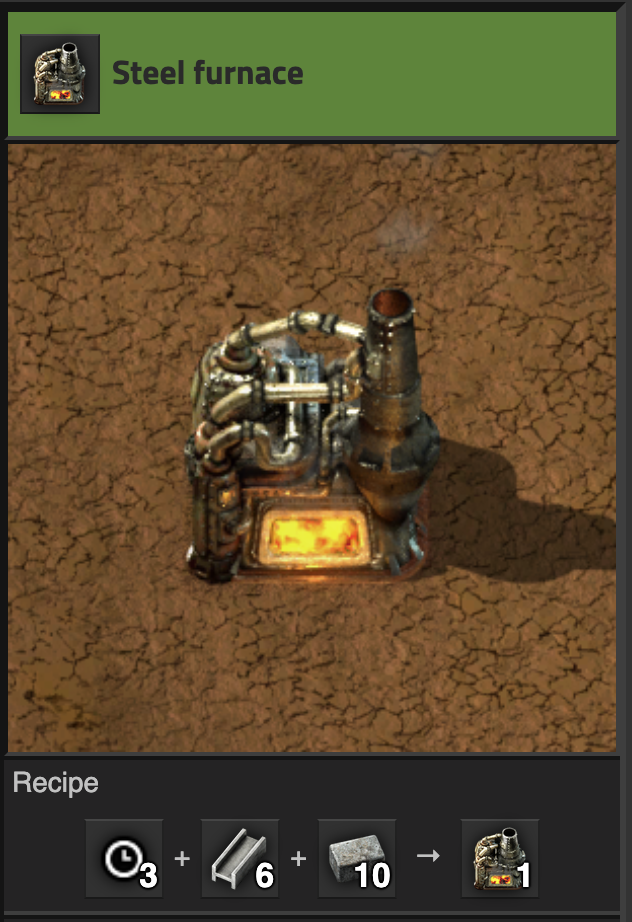
\includegraphics[width=0.5\linewidth]{images/furnace_ex1.png}
        
        \small Figure 1: Building cost
    \end{minipage}
    \hfill
    \vrule
    \hfill
    \begin{minipage}{0.47\linewidth}
        \centering
        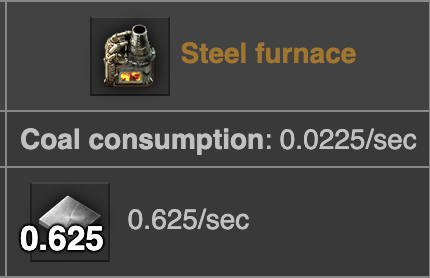
\includegraphics[width=\linewidth]{images/recex1.png}
        
        \small Figure 2: Building input/output
    \end{minipage}
\end{frame}

\begin{frame}{Background: Logistics and bottlenecks}
\begin{itemize}
    \item A part of the difficulty of \factorio{Factorio} are the logistics
    \item Resources must be moved between buildings using belts, inserters, pipes, or similar infrastructure
    \item $\to$ spatial constraints, transport delays, and throughput limits.
    \item Even when the necessary items exist somewhere in the factory, production can stall because the right items do not reach the right machines at the right time
\end{itemize}
\end{frame}

\begin{frame}{Game screenshot}
    \begin{figure}
        \centering
        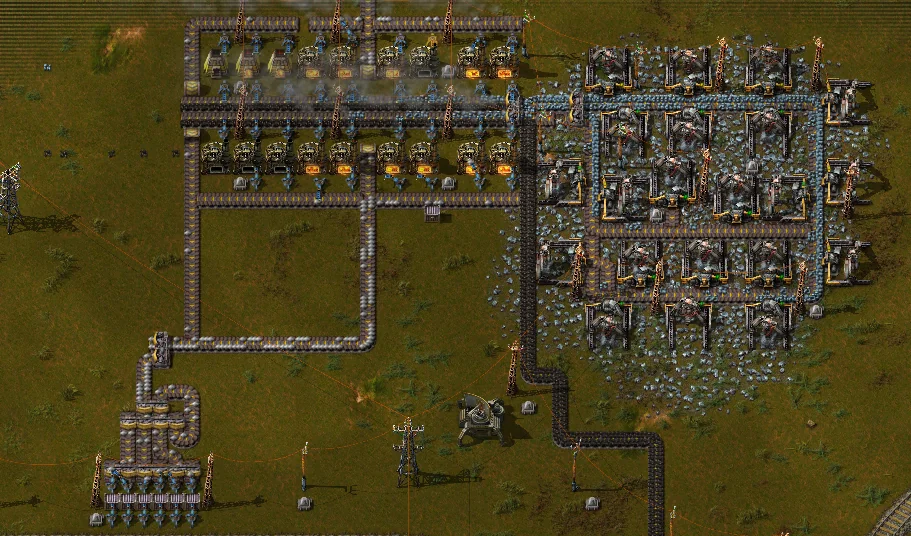
\includegraphics[width=0.75\linewidth]{images/factorio_screenshot1.png}
        \caption{Screenshot of miner+smelter setup.}
        \label{fig:enter-label}
    \end{figure}
\end{frame}

\begin{frame}{Background: Technological progression}
\begin{itemize}
    \item Progression in \factorio{Factorio} is gated by research
    \item Science packs + laboratories $\to$ new technologies (available recipes, buildings)
    \item Early-game production $\to$ advanced outputs
    \item In this project, technological progression through research is \textbf{not} modeled.
\end{itemize}
\end{frame}

\begin{frame}{Modeling overview}
\begin{itemize}
    \item Model \factorio{Factorio} as a discrete-time planning problem using ASP
    \item Focus on temporal scheduling of building and crafting actions
    \item Logistic aspects are not modeled explicitly $\to$ factory regions called \textbf{zones}.
\end{itemize}
\end{frame}

\begin{frame}[fragile]{Static game encoding}
The encoding distinguishes between \textbf{crafting recipes} and \textbf{buildings} representing automated production units.

\vspace{0.4em}
\begin{lstlisting}[language=asp]
% items
item(iron_plate).
item(green_circuit).
item(assembler).

% manual crafting recipe
crafting(assembler).
dur(assembler,1).
crafting_cost(assembler, iron_plate, 100).
crafting_cost(assembler, green_circuit, 30).
crafting_out(assembler, assembler, 10).

% automated building
building(green_circuit_assembler).
dur(green_circuit_assembler, 1).
building_cost(green_circuit_assembler, assembler, 5).
building_in(green_circuit_assembler, iron_plate, 100).
building_in(green_circuit_assembler, electricity, 78).
building_out(green_circuit_assembler, green_circuit, 100).
\end{lstlisting}
\end{frame}

\begin{frame}{Simplifications}
The model uses fixed-length time horizons (e.g., 20-30 steps), each step corresponds to 30 seconds of in-game time

\vspace{0.6em}
\begin{itemize}
    \item Spatial placement is abstracted away and replaced by zones.
    \item Logistic infrastructure is not modeled explicitly.
    \item All recipes are available from the start
    \item Recipes are treated at aggregate rates per step
    \item At most one manual crafting action and one building action per step
\end{itemize}
\end{frame}

\begin{frame}[fragile]{Actions and delayed completion}
At each step, the player may start up to one crafting action and one building action. Once started, the respective activity channel remains occupied until the duration expires.

\vspace{0.4em}
\begin{lstlisting}[language=asp]
% at most one craft and one build action per step
0 { act(craft(C), STEP) : crafting(C), dur(C, _) } 1
  :- step(STEP), not busy(craft, STEP).

0 { act(build(B, Z), STEP) : building(B), zone(Z),
    dur(B, _), can_build(B, Z) } 1
  :- step(STEP), not busy(build, STEP).

% activity channels stay occupied until the duration expires
busy(craft, STEP) :- step(STEP), act(craft(C), STEP0),
  dur(C, D), STEP > STEP0, STEP < STEP0 + D.

% completion time
finish(craft(C), TIME) :- time(TIME), act(craft(C), STEP0),
  dur(C, D), TIME = STEP0 + D.
\end{lstlisting}

\vspace{0.2em}
{\small Craft and build channels are handled symmetrically in the full encoding.}
\end{frame}

\begin{frame}{Zones}
\begin{columns}[T,onlytextwidth]
\column{0.48\textwidth}
\begin{itemize}
    \item The factory is partitioned into \textbf{zones}.
    \item Each zone contains a fixed number of \textbf{slots}.
    \item A slot may be assigned at most one building type.
    \item A building type may appear in at most one slot per zone.
    \item The slot assignment is fixed over the horizon.
    \item \texttt{building\_count(B,Z,T)} represents the installed capacity.
\end{itemize}

\column{0.52\textwidth}
\centering
\IfFileExists{images/zones_new.png}{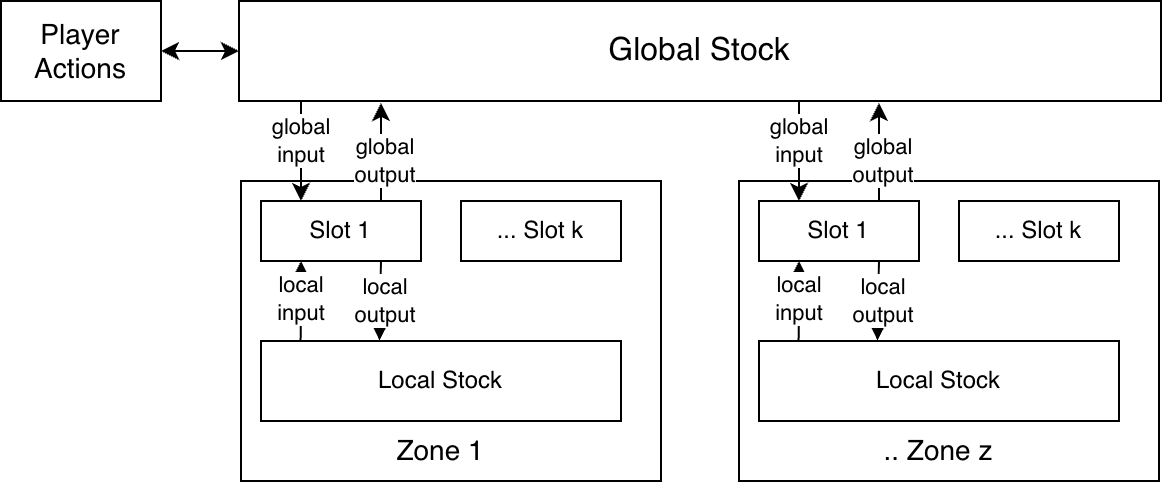
\includegraphics[width=\linewidth]{images/zones_new.png}}{\fbox{\parbox[c][0.45\textheight][c]{0.9\linewidth}{\centering Figure referenced from the article:\\[0.4em]\texttt{images/zones\_new.png}}}}

\vspace{0.3em}
{\scriptsize Zone resource flow model.}
\end{columns}
\end{frame}

\begin{frame}[fragile]{Zones}
\begin{lstlisting}[language=asp]
zone(1..num_zones).
slot(1..num_slots).
available_index(1..num_slots+1).
next_zone(Z, Z+1) :- zone(Z), zone(Z+1).

% at most one building type per slot
0 { slot_map(Z, S, B) : building(B) } 1 :- zone(Z), slot(S).

% a building type may occupy at most one slot per zone
:- slot_map(Z, S1, B), slot_map(Z, S2, B), S1 != S2.

% keep used slots left-aligned
has_assignment(Z, S) :- slot_map(Z, S, _).
:- has_assignment(Z, S+1), not has_assignment(Z, S), slot(S).

% build actions only for assigned building types
can_build(B, Z) :- building(B), zone(Z), slot_map(Z, _, B).
\end{lstlisting}
\end{frame}

\begin{frame}{Time model and state variables}
\begin{itemize}
    \item The factory is modeled over a fixed horizon with \texttt{time(0..H)} and \texttt{step(0..H-1)}.
    \item A \textbf{time point} represents a snapshot of the state.
    \item A \textbf{step} represents the transition between two consecutive snapshots.
    \item One step corresponds to 30 seconds of in-game time.
\end{itemize}

\vspace{0.6em}
At each time point \(T\), the relevant part of the state is:
\begin{itemize}
    \item \texttt{global\_stock(I,T)}: global stock of item \(I\),
    \item \texttt{stock(I,Z,T)}: local stock of item \(I\) in zone \(Z\),
    \item \texttt{building\_count(B,Z,T)}: number of buildings of type \(B\) in zone \(Z\).
\end{itemize}
\end{frame}

\begin{frame}[fragile]{Intra-step resource allocation: initialization}
Within one step, multiple buildings may compete for the same limited resources. To remove ambiguity, the model fixes the order in which zones and slots gain access to available resources.

\vspace{0.4em}
\begin{lstlisting}[language=asp]
uses_build_resource(I, T) :- act(build(B, _), T), building_cost(B, I, _).
uses_craft_resource(I, T) :- act(craft(C), T), crafting_cost(C, I, _).

% each zone starts with its local stock available to slot 1
&sum { local_available(I, Z, 1, T); -stock(I, Z, T) } = 0
  :- item(I), zone(Z), step(T).

% first slot of first zone receives remaining global stock
&sum { global_available(I, 1, 1, T); -global_stock(I, T);
       cost_build(I, T); cost_craft(I, T) } = 0
  :- item(I), step(T).

% available output space
&sum { local_space(I, Z, 1, T); stock(I, Z, T) } = Cap
  :- item(I), zone(Z), step(T), init_local_cap(I, Z, Cap).
&sum { global_space(I, 1, 1, T); global_stock(I, T) } = Cap
  :- item(I), step(T), init_global_cap(I, Cap).
\end{lstlisting}
\end{frame}

\begin{frame}[fragile]{Core intra-step flow constraints}
For each occupied slot, the solver chooses a utilization value between zero and installed capacity. This utilization is constrained by available inputs and available output space.

\vspace{0.4em}
\begin{lstlisting}[language=asp]
&dom{0..max_val} = slot_utilization(Z, S, T) :- zone(Z), slot(S), step(T).

% utilization cannot exceed installed capacity
&sum { slot_utilization(Z, S, T); -building_count(B, Z, T) } <= 0
  :- slot_map(Z, S, B), step(T).

% required inputs = recipe demand * utilization
&sum { input_from_local(I, Z, S, T); input_from_global(I, Z, S, T);
       -Qty*slot_utilization(Z, S, T) } = 0
  :- slot_map(Z, S, B), building_in(B, I, Qty), step(T).

% produced outputs = recipe output * utilization
&sum { output_to_local(I, Z, S, T); output_to_global(I, Z, S, T);
       -Qty*slot_utilization(Z, S, T) } = 0
  :- slot_map(Z, S, B), building_out(B, I, Qty), step(T).
\end{lstlisting}

\vspace{0.2em}
{\small Availability and storage-space constraints bound these flows in the full encoding.}
\end{frame}

\begin{frame}[fragile]{Propagation and state transition}
After a slot's utilization is fixed, the remaining local resources, global resources, and output space are passed forward. At the end of the step, the model fixes the state at time \(T+1\).

\vspace{0.4em}
\begin{lstlisting}[language=asp]
% pass remaining resources to next slot
&sum { local_available(I, Z, S+1, T); -local_available(I, Z, S, T);
       input_from_local(I, Z, S, T) } = 0
  :- item(I), zone(Z), slot(S), step(T).

% building capacity increases when build action finishes
&sum { building_count(B, Z, T+1); -building_count(B, Z, T) } = 1
  :- building(B), zone(Z), step(T), slot_map(Z, _, B), finish(build(B, Z), T).

% local stock at T+1 = remaining local availability + outputs to local stock
&sum { stock(I, Z, T+1); -local_available(I, Z, num_slots+1, T);
       -output_to_local(I, Z, S, T) : slot(S) } = 0
  :- item(I), zone(Z), step(T).

% global stock at T+1 = remaining global availability + outputs to global + craft yield
&sum { global_stock(I, T+1); -global_available(I, num_zones, num_slots+1, T);
       -output_to_global(I, Z, S, T) : zone(Z), slot(S);
       -yield_craft(I, T+1) } = 0 :- item(I), step(T).
\end{lstlisting}
\end{frame}

\begin{frame}[fragile]{Optimization objective}
The model does not force greedy utilization per slot. Instead, utilization is selected by the solver subject to the constraints and the optimization objective.

\vspace{0.6em}
\begin{lstlisting}[language=asp]
% want factories to run as much as possible, consume local resources first
&maximize {
 100*slot_utilization(Z, S, T) : zone(Z), slot(S), step(T);
 -1*input_from_global(I, Z, S, T) : item(I), zone(Z), slot(S), step(T)
}.
\end{lstlisting}

\vspace{0.6em}
\begin{itemize}
    \item First priority: keep factories running as much as possible.
    \item Second priority: prefer local resource usage over the global pool.
\end{itemize}
\end{frame}

\begin{frame}[fragile]{Planning from existing game states}
An instance specifies the starting global stock, local zone stocks, installed buildings, and one or more target conditions.

\vspace{0.3em}
\begin{columns}[T,onlytextwidth]
\column{0.48\textwidth}
\begin{lstlisting}[language=asp]
#const horizon = 15.
#const num_zones = 2.
#const num_slots = 8.

init_global_stock(electricity, 500).
init_global_stock(coal, 500).
init_building_count(offshore_pump, 1, 1, 1).
init_building_count(power_plant_small, 1, 2, 2).
init_building_count(coal_mine, 1, 3, 1).
init_building_count(iron_mine, 1, 4, 1).

goal_item(green_circuit, 100).
goal_building(green_circuit_assembler, 1).
\end{lstlisting}

\column{0.50\textwidth}
\begin{itemize}
    \item Run with \textbf{clingcon}.
    \item Output is either \textbf{UNSAT} or a sequence of actions achieving the goals within the horizon.
    \item green\_circuit.lp
    \begin{itemize}
        \item \(H = 14\): \textbf{UNSAT}
        \item \(H = 15\): viable solution
    \end{itemize}
\end{itemize}

\vspace{0.4em}
\begin{lstlisting}[language=bash]
$ clingcon --stats model.lp game.lp \
  instances/{name} --opt-mode=opt \
  -n 0 --quiet=1 -t 64 --time 1200
\end{lstlisting}
\end{columns}
\end{frame}
\begin{frame}[fragile]{Output}
\textbf{Solver output (excerpt):}

\begin{lstlisting}[language=asp]
Answer: 1 (Time: 227.251s)

act(craft(assembler),10)
act(craft(copper_cable),5) act(craft(copper_cable),6)
...
act(build(iron_smelter,2),3) act(build(iron_smelter,2),4)
act(build(steel_smelter,2),10)
...
finish(craft(stone_furnace),4) finish(craft(stone_furnace),5)
finish(craft(stone_furnace),14)
...
finish(build(copper_cable_assembler,2),12)
finish(build(steel_smelter,2),11)
...
slot_map(1,1,offshore_pump) slot_map(1,2,power_plant_small)
slot_map(2,8,battery_chemical_plant)
\end{lstlisting}
\end{frame}
\begin{frame}{}
    \begin{figure}
        \centering
        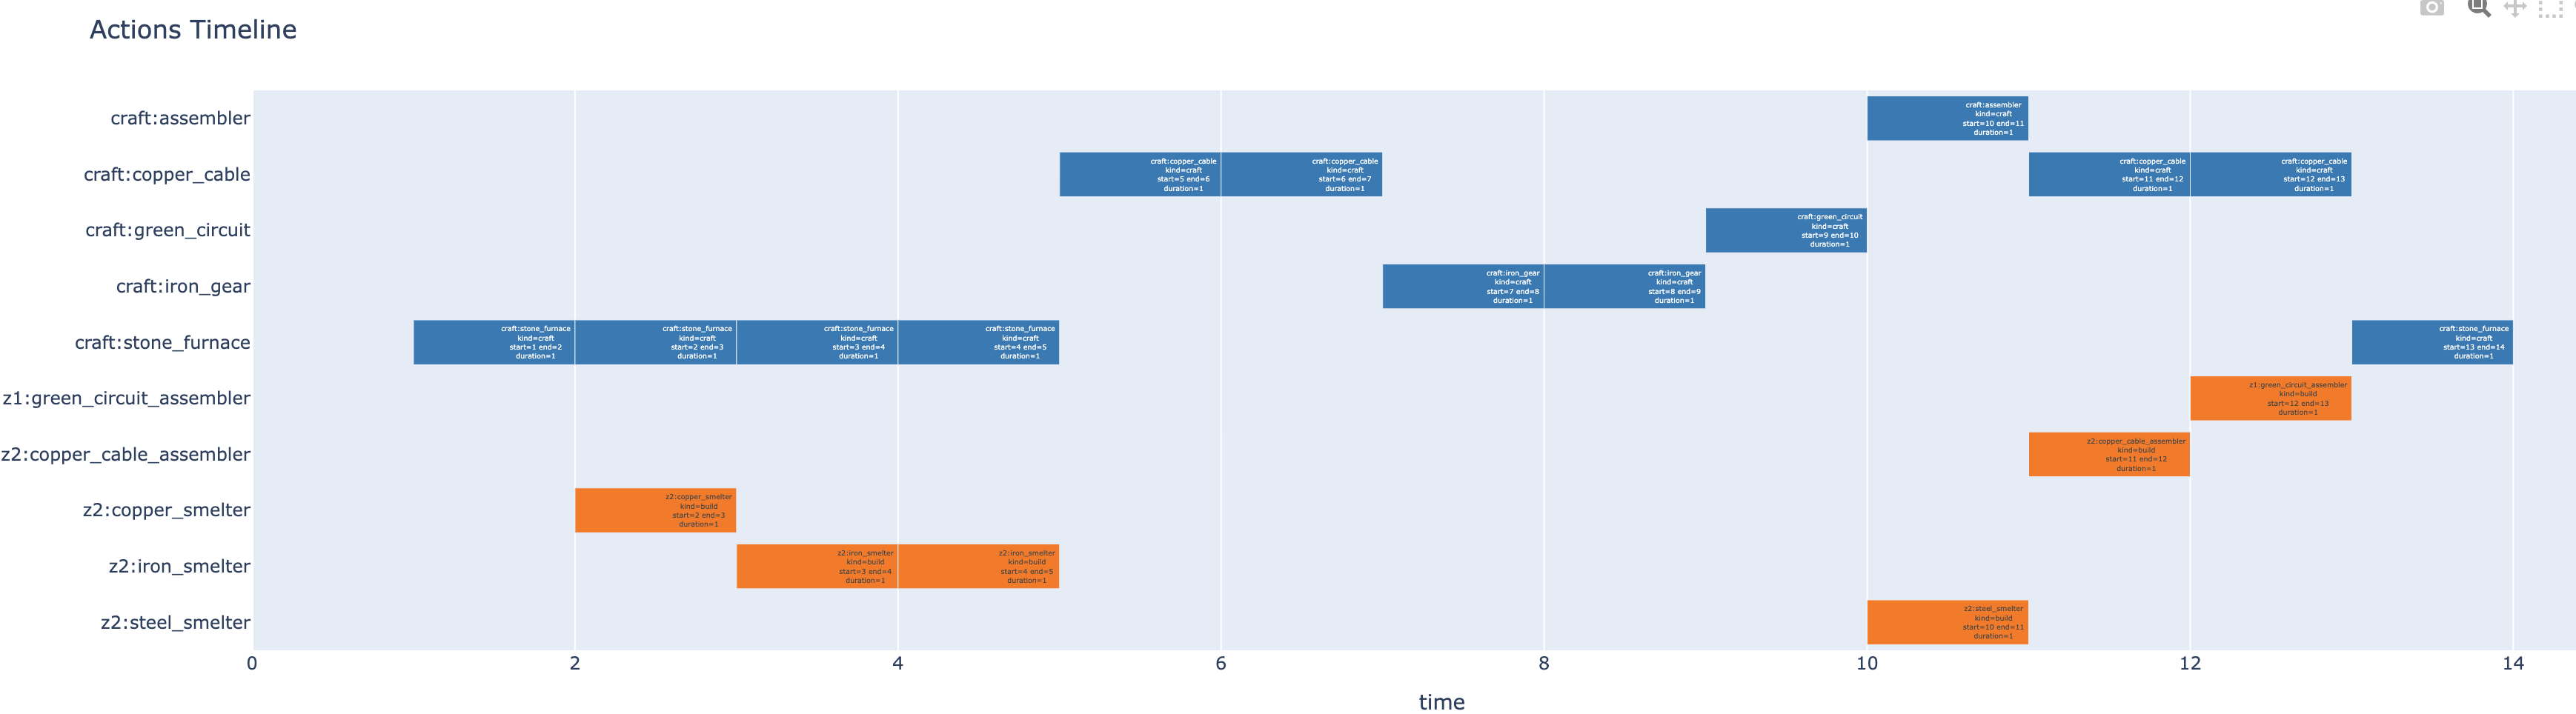
\includegraphics[width=1\linewidth]{images/timelinegreenc.png}
        \caption{Action timeline}
        \label{fig:enter-label}
    \end{figure}
\end{frame}
\begin{frame}{Conclusion}
\begin{itemize}
    \item Planning model for a simplified version of \factorio{Factorio}
    \item Test whether a goal is reachable within a given horizon
    \item Find action sequences that achieve the specified objectives
\end{itemize}

\vspace{0.8em}
\centering
\Large Questions?
\end{frame}

\end{document}
